\chapter{Interaction of Multiple Selected Loci}

Consider two biallelic loci segregating for $A/a$ and $B/b$. There are four haplotypes, $AB$, $Ab$, $aB$, $ab$, which for simplicity we label 1-4. The frequency of our four haplotypes are $x_1$, $x_2$, $x_3$, and $x_4$. Each individual has a genotype consisting of two haplotypes; we label $w_{ij}$ the fitness of an individual with the genotype made up of haplotype $i$ and $j$ (we assume that $w_{ij}=w_{ji}$, i.e. there are no parent of origin effects). Assuming that these fitnesses reflect differences due to viability selection, and that individuals mate at random, we can write the following table of our genotype proportions after selection:\\
\begin{center}
\begin{tabular}{c|cccc}
         & $AB$			& $Ab$				& $aB$				& $ab$\\
\hline
$AB$ & $w_{11} x_1^2$ 	& $w_{12} 2 x_1 x_2$  	& $w_{13} 2 x_1 x_3$ 	& $w_{14} 2 x_1 x_4$ \\
$Ab$ & $\bullet$ 	  	& $w_{22} x_2^2$ 	  	& $w_{23} 2 x_2 x_3$  	& $w_{24} 2 x_2 x_4$ \\  
$aB$ & $\bullet$ 		& $\bullet$ 			& $w_{33} x_3^2$ 	  	& $w_{34} 2 x_3 x_4$ \\  
$ab$ & $\bullet$ 		& $\bullet$			& $\bullet$ 			&  $w_{44} x_4^2$ \\
\end{tabular}
\end{center}
This follows from assuming that our haplotypes are brought together at random (HWE), then discounted by their fitnesses. Our mean fitness $\bar{w}$ is the sum of all the entries in the table, so dividing by $\bar{w}$ normalizes the complete table to sum to one. The frequency of the $AB$ haplotype ($1$) in the next generation of gametes is
\begin{equation}
x_1' = \frac{\big( w_{11} x_1^2 +	 \half w_{12} 2 x_1 x_2  + \half w_{13} 2x_1 x_3  +	 \half (1-r) w_{14} 2 x_1 x_4 + \half r w_{23} 2 x_2 x_3   \big)}{ \bar{w} } \label{eqn:hapfreq}
\end{equation}
This is a bit of a mouthful, but each of the terms is easy to understand. Each of the HWE genotype frequencies (e.g. $2x_1x_2$) is weighted by its fitness relative to the mean fitness ($w_{ij}/\bar{w}$), and by its probability of transmitting the AB haplotype to the next generation. For example, $AB/Ab$ individuals (1/2) transmit the $AB$ haplotype only half the time. The final two terms include the recombination fraction ($r$). The first term involving recombination refers to the $AB/ab$ genotype (1/4), who with probability $(1-r)/2$ transmits a non-recombinant $AB$ haplotype to the gamete. Similarly, the second term refers to the  $Ab/aB$ genotype; a proportion $r/2$ of its gametes carry the recombinant $AB$ haplotype. 

In the single locus case, we defined the marginal fitness of an allele. Here it will help us to define the marginal fitness of the $i^{th}$ haplotype:
\begin{equation}
\bar{w}_i = \sum_{j=1}^4 w_{ij} x_j
\end{equation}
This is the fitness of the $i^{th}$ haplotype averaged over all of the \ec{diploid} genotypes it could occur in, weighted by their probability under random mating. Using this notation, and with some rearrangement of equation \eqref{eqn:hapfreq}, we obtain
\begin{equation}
x_1' = \frac{x_1\bar{w}_1 - w_{14} r D}{\bar{w}}
\end{equation}
Here we have assumed that $w_{23}=w_{14}$, i.e. that the fitness of $AB/ab$ individuals is the same as $Ab/aB$ individuals (i.e. that fitness depends only on the alleles carried by an individual, and not on which chromosome they are carried; this assumption is sometimes called no {\it cis}-epistasis). 

We can then write the change in the frequency of our $1$ haplotype as 
\begin{equation}
\Delta x_1= \frac{x_1(\bar{w}_1-\bar{w}) -r w_{14} D}{\bar{w}}
\end{equation}
Generalizing this result, we write the change in \ec{any haplotype i from} our set of four haplotypes as
\begin{equation}
\Delta x_i= \frac{x_i(\bar{w}_i-\bar{w}) \pm r w_{14} D}{\bar{w}}
\end{equation}
where the coupling haplotypes 1 and 4 use $+D$ and repulsion haplotypes 2 and 3 use $-D$. \erin{I'm confused about the signs +/- here. For haplotype 1 above you used -rw14D but here you're saying it's +D. Also, why doesn't the sign of D itself take care of the +/- (I think this second part is just my own confusion, but the first part doesn't seem to match between the equation above and your text)} Note that the sum of these four $\Delta x_i$ is zero, as our haplotype frequencies sum to one.

So the change in the frequency of a haplotype (e.g. AB, haplotype 1) is determined by the interplay of two factors: First, the extent to which  the marginal fitness of our haplotype is higher (or lower) than the mean fitness of the population (the magnitude and sign of $(\bar{w}_1-\bar{w})/\bar{w}$). Second, whether there is a deficit or any excess of our haplotype compared to linkage equilibrium (the magnitude and sign of $D$), modified by the strength of recombination. This tension between selection promoting particular haplotypic combinations, and recombination breaking up overly common haplotypes is the key to a lot of interesting dynamics and evolutionary processes.

\section{Types of interaction between selection and recombination}

\gc{To illustrate these ideas we make use of Muller diagrams \citep{muller1932some}, where we visualize the allele dynamics in terms of a plot of thestack frequencies over time.}

\paragraph{The hitchhiking of deleterious alleles}
\begin{figure}
\begin{center}
  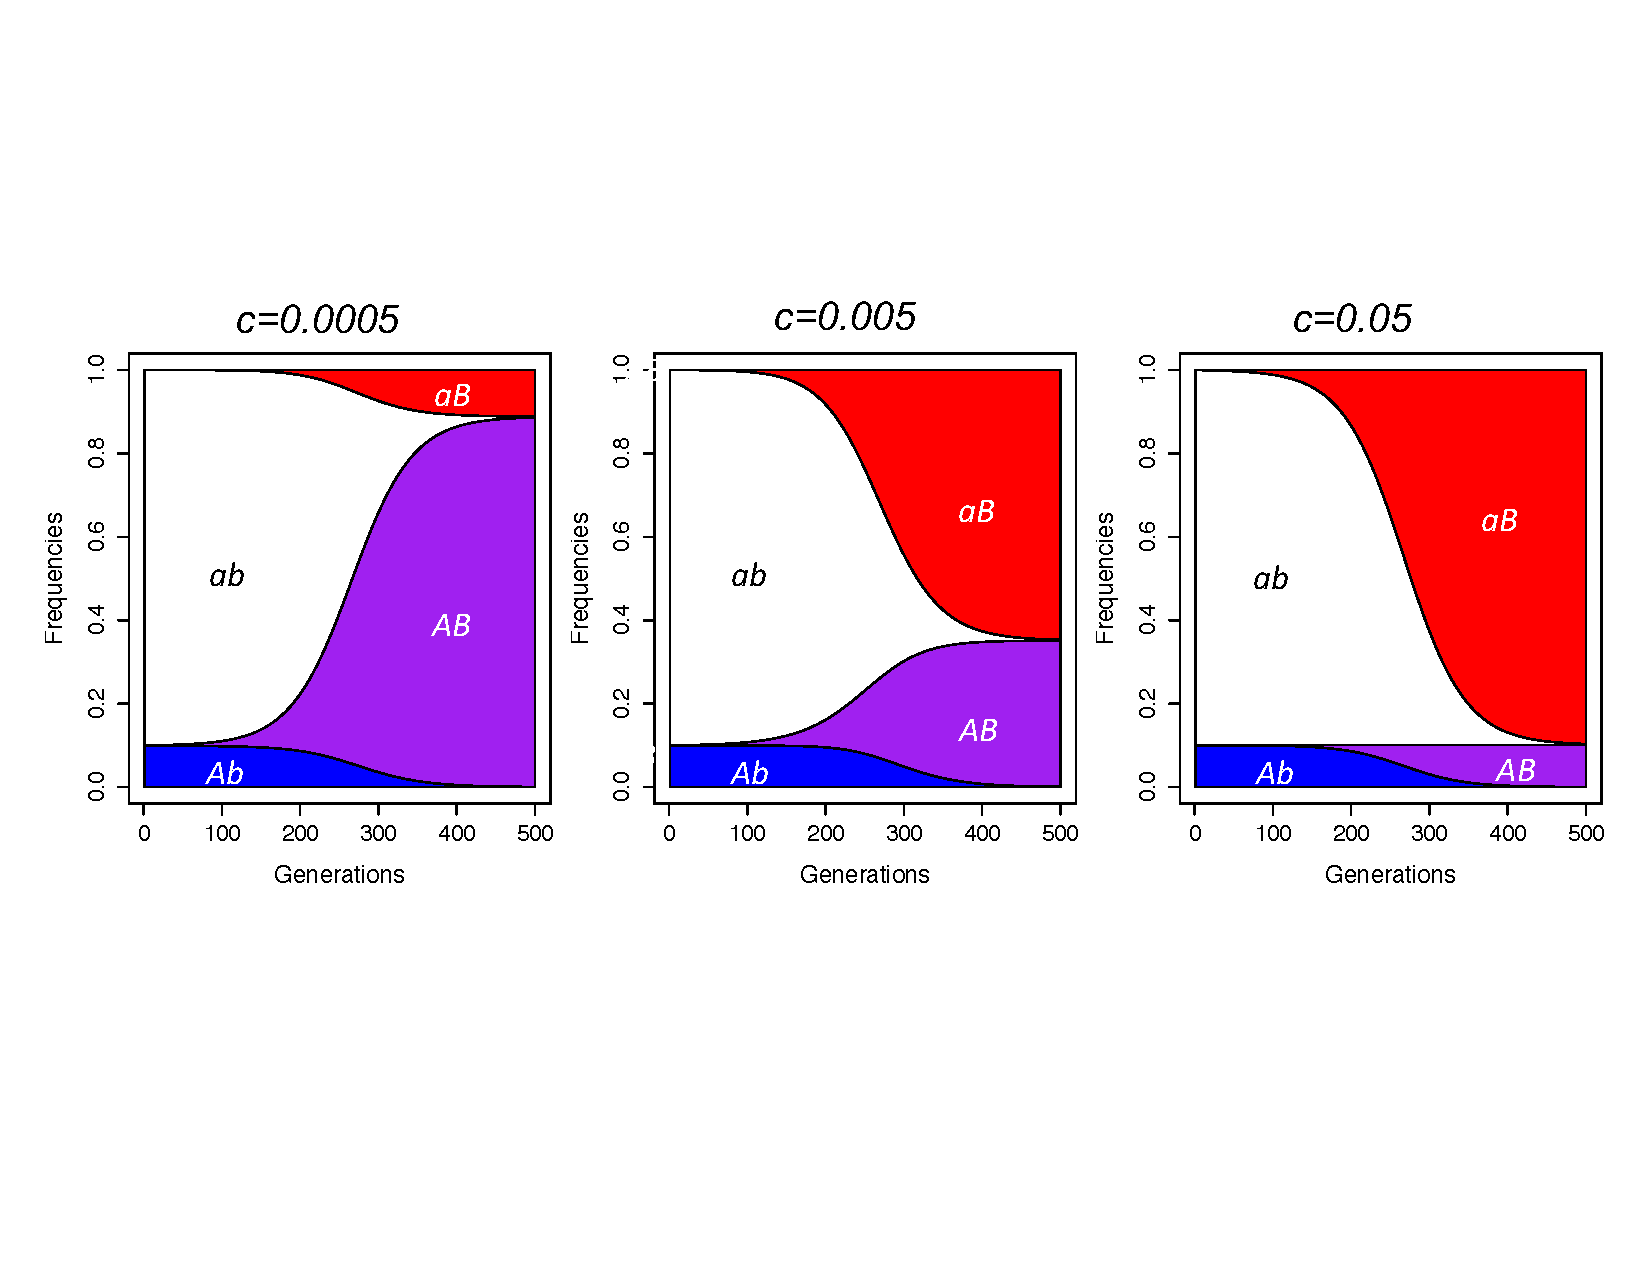
\includegraphics[width = 0.9 \textwidth]{figures/selection_recom_interaction/Neutral_Hitchhiking_labeled.pdf}
\end{center}
\caption{A beneficial mutation $B$ arises on the background of a neutral allele whose initial frequency is $p_A=10\%$. The beneficial allele has a strong, additive selection coefficient of $hs=0.05$.} \label{fig:Neutral_HH}  %é
\end{figure}
Let's start by revisiting our neutral hitchhiking in this two locus setting in the previous chapter we saw that neutral alleles can hitchhike along with our selected allele if they are tightly linked enough. Figure \ref{fig:Neutral_HH}  shows the frequency trajectories of the various haplotypes for neutral allele ($A$) that is present at $10\%$ frequency in the population when our beneficial allele ($B$) arises on its background. When the recombination rate ($r$) is low between the loci, $A$ gets to hitchhike to high frequency, but for higher recombination rates it only gets dragged to intermediate frequencies. For the highest recombination rate shown ($r \approx s$) the neutral allele's dynamics ($p_{Ab}+p_{AB}$) are barely changed at all, as it recombines on and off the sweeping allele frequently and so barely perceives the sweep. 

\paragraph{The hitchhiking of deleterious alleles}
Deleterious alleles can also hitchike along with beneficial mutations if they are not too deleterious compared to the benefits offered by the selected allele. Again our allele $A$ is at $10\%$ frequency in the population in Figure \ref{fig:deleterious_HH}, but this time it is deleterious and so initially decreasing in frequency across the generations when the beneficial mutation ($B$) arises on its background. If the loci are tightly linked, and A were too deleterious, B would never get to take off in the population.   However, if the benefits of B outweighs the cost of A, even in the case of no recombination between our loci, allele $A$ gets to hitchhike to fixation and merely slows down $B$'s rate of increase and their combined fitness is reduced. With moderate amounts of recombination between the loci, our deleterious starts to hitchhike but before it can get to fixation the beneficial allele manages to recombine off its background. This recombinant aB haplotype, which has higher fittest as it lacks the deleterious allele, now sweeps through the population displacing the AB haplotype. For higher recombination events we have to wait less long for a recombination to breakup the hitchhiking deleterious allele, so the adaptive allele easily escapes its background.
For the purposes of illustration here we've used a relatively common deleterious allele, but in reality these alleles will likely be often be rare in the population and at mutation selection balance. If they are rare it is likely that a beneficial mutation arises on a specific deleterious allele's background, but as we have seen there are likely going to be many rare deleterious alleles in the population so it is likely that a beneficial mutations may often have to contend with deleterious hitchhikers. 
\begin{figure}
\begin{center}
  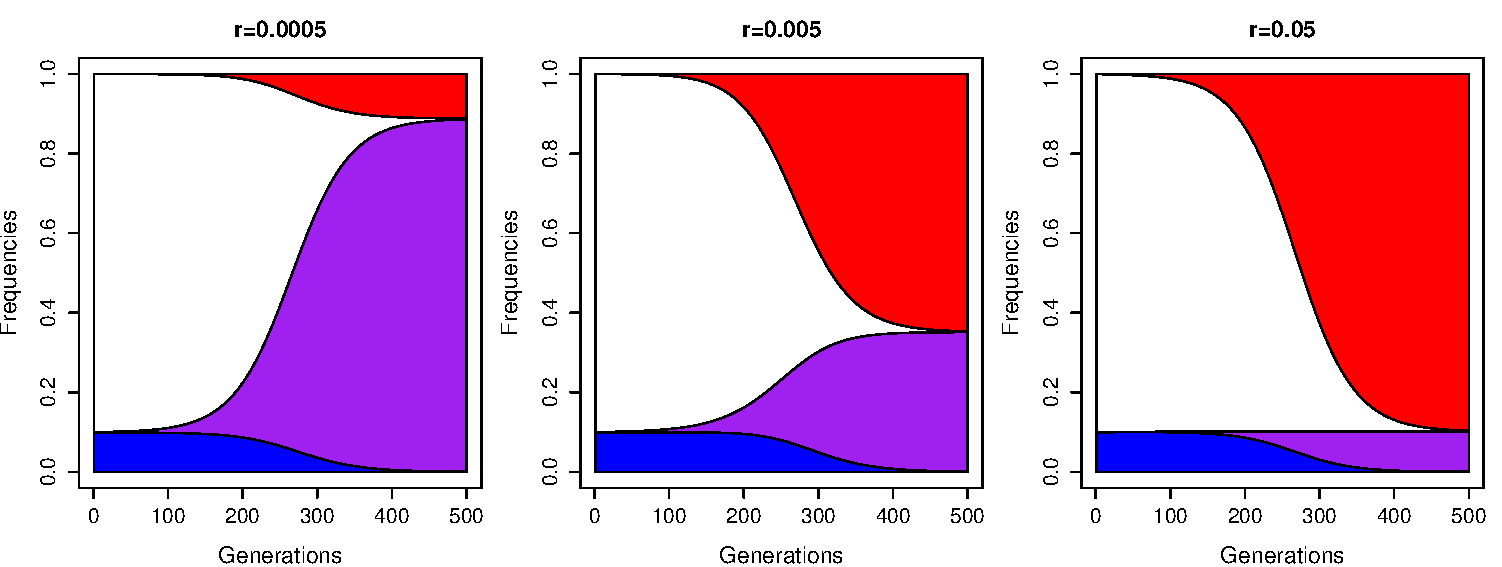
\includegraphics[width = 0.9 \textwidth]{figures/selection_recom_interaction/Deleterious_Hitchhiking.pdf}
  \caption{} \label{fig:deleterious_HH}  %é
  \end{center}
\end{figure}


\begin{figure*}
\begin{center}
  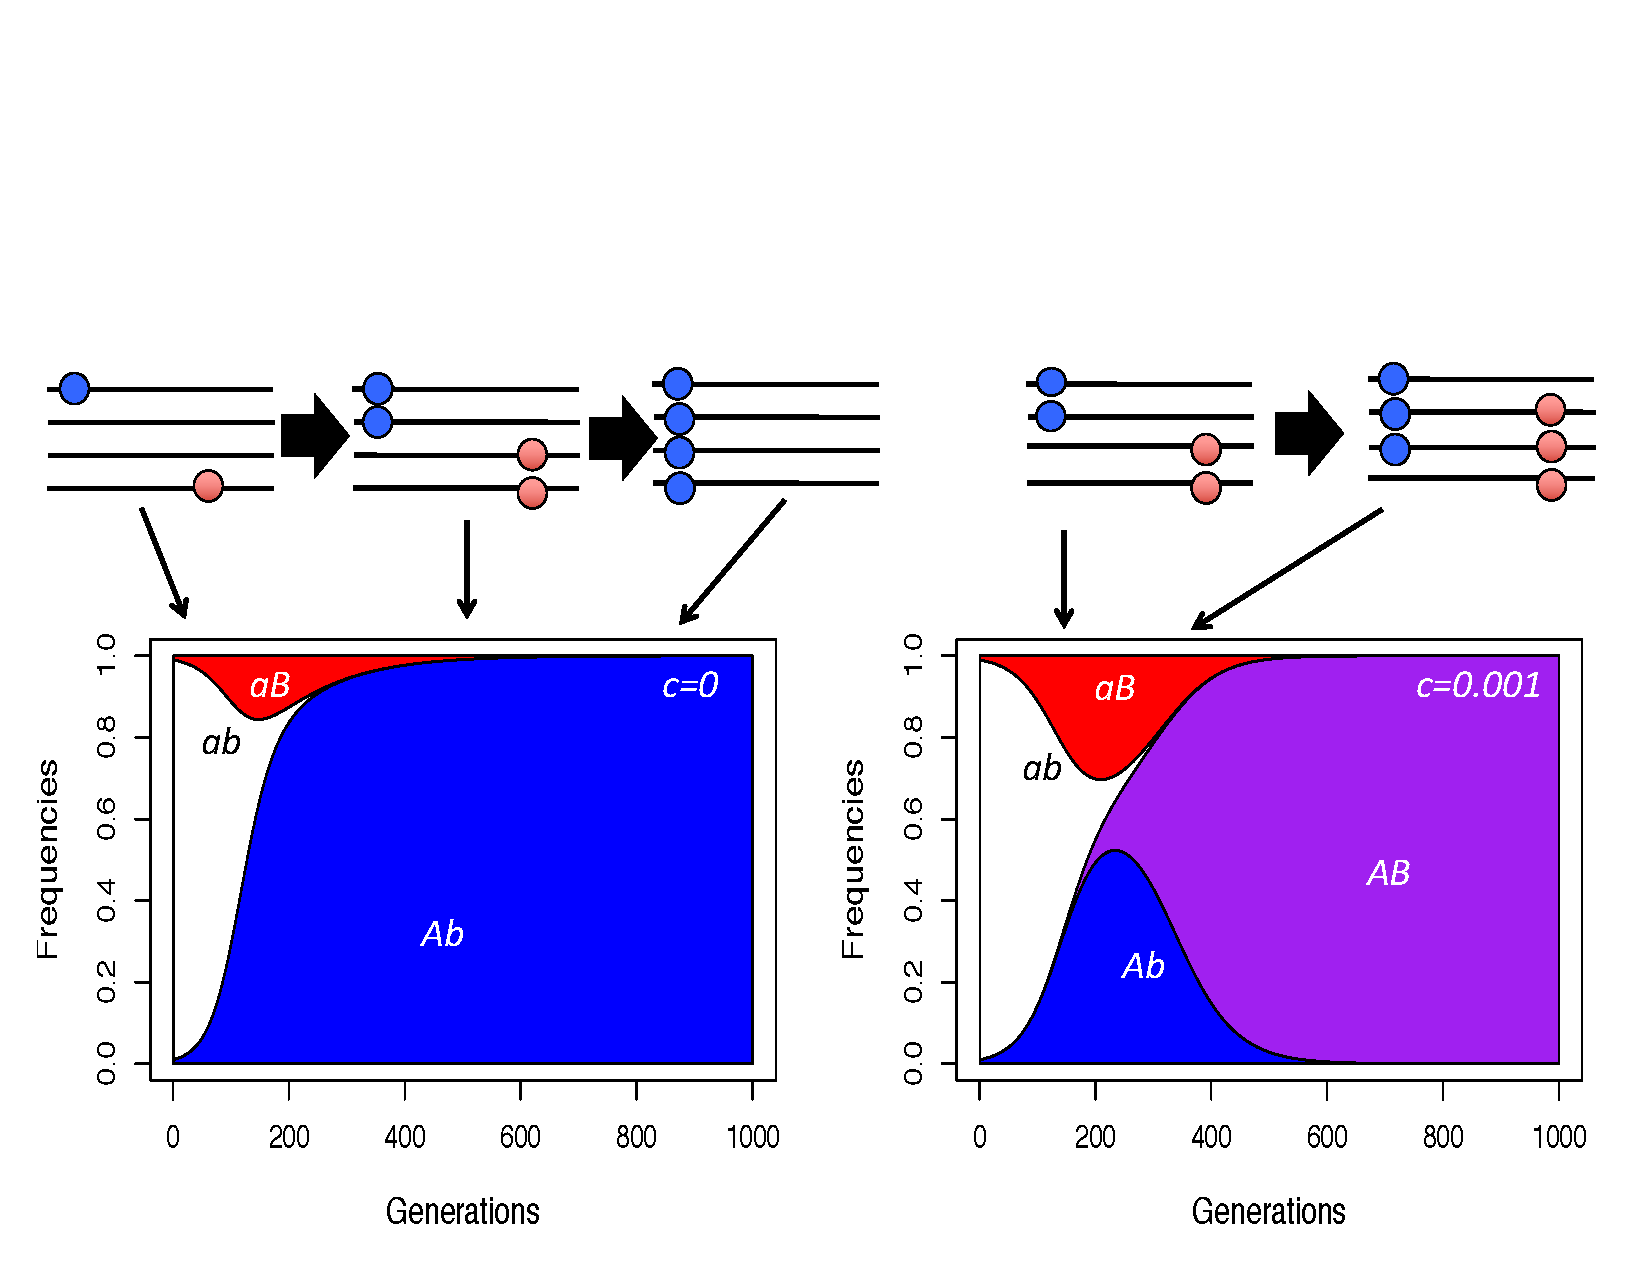
\includegraphics[width = 0.8 \textwidth]{figures/selection_recom_interaction/Interference_w_haps.pdf}
\end{center}
\caption{Interference between two positively selected alleles. {\bf Left)} the red and blue (A and B) beneficial alleles arise on different haplotypes. They rise in frequency, but in the absence of recombination only one can fix. This is shown in a Muller diagram, where $p_{AB}$ is initially set to zero. {\bf Right)} In the presence of recombination the population can generate the recombinant (AB) haplotype, which can subsequently fix.} \label{fig:Interference}  %é
\end{figure*}
\paragraph{Clonal interference between favourable alleles.}
When rates of sex and recombination are zero, or very low, positively selected alleles can prevent each other reach fixation and so the rate of adaptation can be slowed.
In the absence of sex and recombination, when two positively selected alleles arise on different genetic backgrounds in the population they cannot both fix (left side of Figure \ref{fig:Interference}). They can initially increase in frequency, but neccessarily compete with each other when they become common. This is called selective interefence, or sometime clonal interference. If one of the alleles has a much larger selection coefficient it will fix, forcing the other allele from the population, but when they are relatively equally matched it may take some time for this situation to resolve itself resulting in a traffic jam in the population. Thus in an asexual adaptive alleles necessarily have to fix sequentually. However, with even a small amount of recombination beneficial alleles can recombine on to each others background, allowing them to fix in parallel (right side of  Figure \ref{fig:Interference}).   

\begin{marginfigure}
\begin{center}
  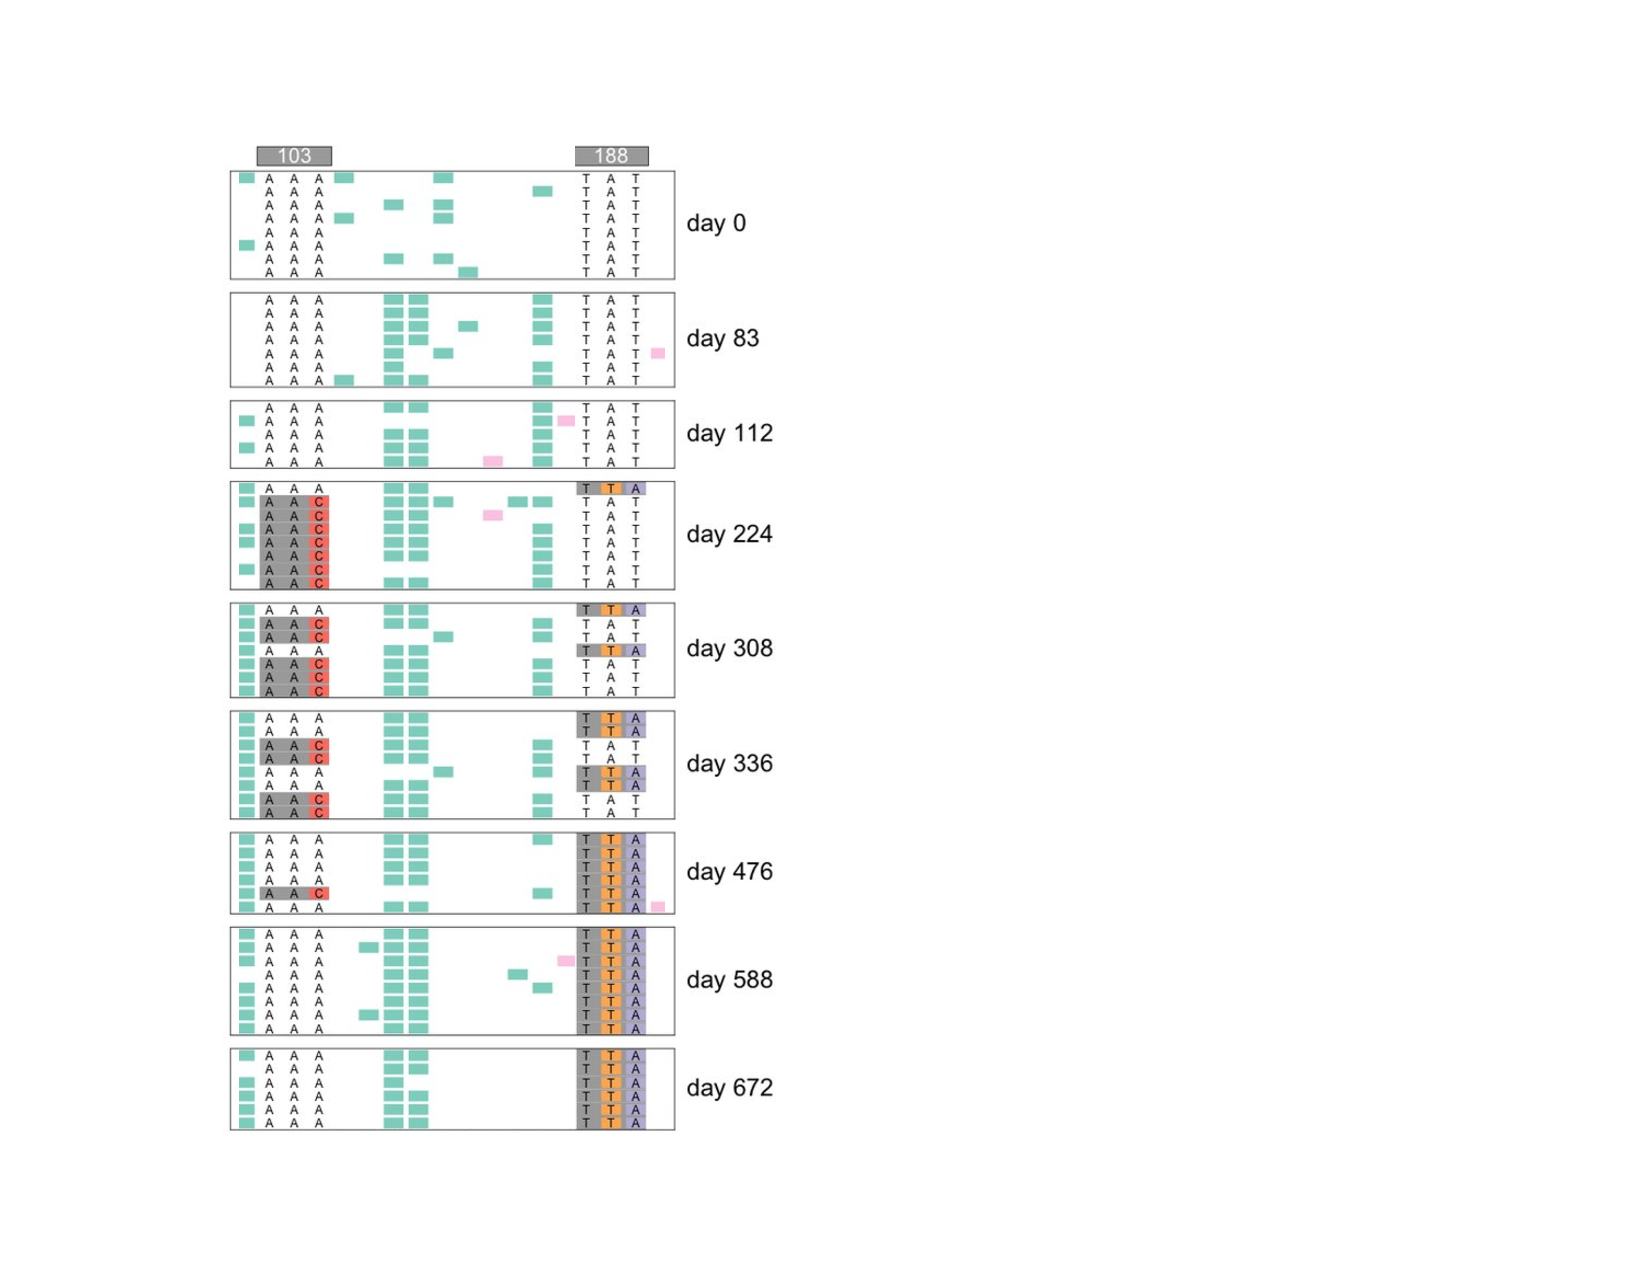
\includegraphics[width =  \textwidth]{Journal_figs/recom_selection/Pleuni_HIV_interference/Trimmed_HIV_interference}  %DdwdkVeVMAA7t-V.jpg}
\end{center}
\caption{HIV sequences from a patient over the course of drug treatment in the retrotransposase coding region. Figure cropped from \citet{Williams548198}, \PLOSccBY.} \label{fig:HIV_interference}  %é
\end{marginfigure}
Given the rapid evolution of HIV we can see interference taking place over very short time periods indeed. HIV uses its reverse transcriptase (RT) gene to write itself from an RNA virus into its host's DNA, allowing HIV to hijack the hosts regulatory machinery, a critical part of its life cycle. One of the early HIV drugs was Efavirenz, which inhibits HIV's RT protein. Sadly, mutations are common in the RT HIV gene, and these mutations, in the presence of the drug, confer a profound fitness advantage, allowing them to spread through the HIV population in patients undergoing anti-HIV treatment. In Figure \ref{fig:HIV_interference} we see that by day 224 after the start of drug treatment two different drug-resistance amino-acid changes beginning to spread within a patient (also shown as a Muller diagram in Figure \ref{fig:HIV_interference_M}). Because these alleles occur on different genetic backgrounds, with little chance for genetic exchange between them, they interfer in each other progress as they compete to fix within the population. Eventually the amino acid change at site 188 wins out. 

\begin{figure}
\begin{center}
  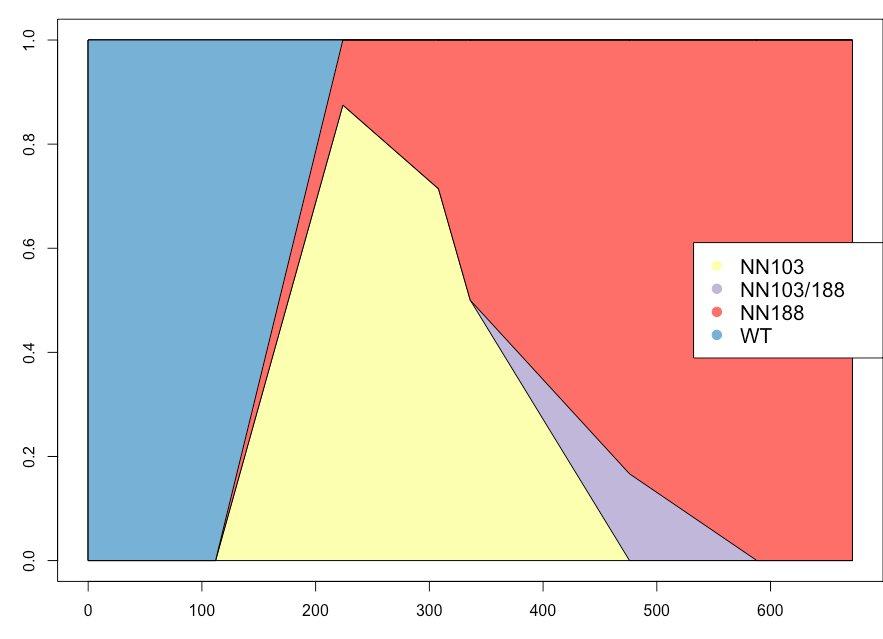
\includegraphics[width = \textwidth]{Journal_figs/recom_selection/Pleuni_HIV_interference/DdweQyxU0AA7mXe.jpg}
\end{center}
\caption{Muller plot of the drug resistance interference dynamics from Figure \ref{fig:HIV_interference}. Figure from \citet{Williams548198}, \PLOSccBY.} \label{fig:HIV_interference_M}  %é
\end{figure}


\paragraph{An example of the costs of asexuality.}


\begin{marginfigure}[-3cm]
\begin{center}
  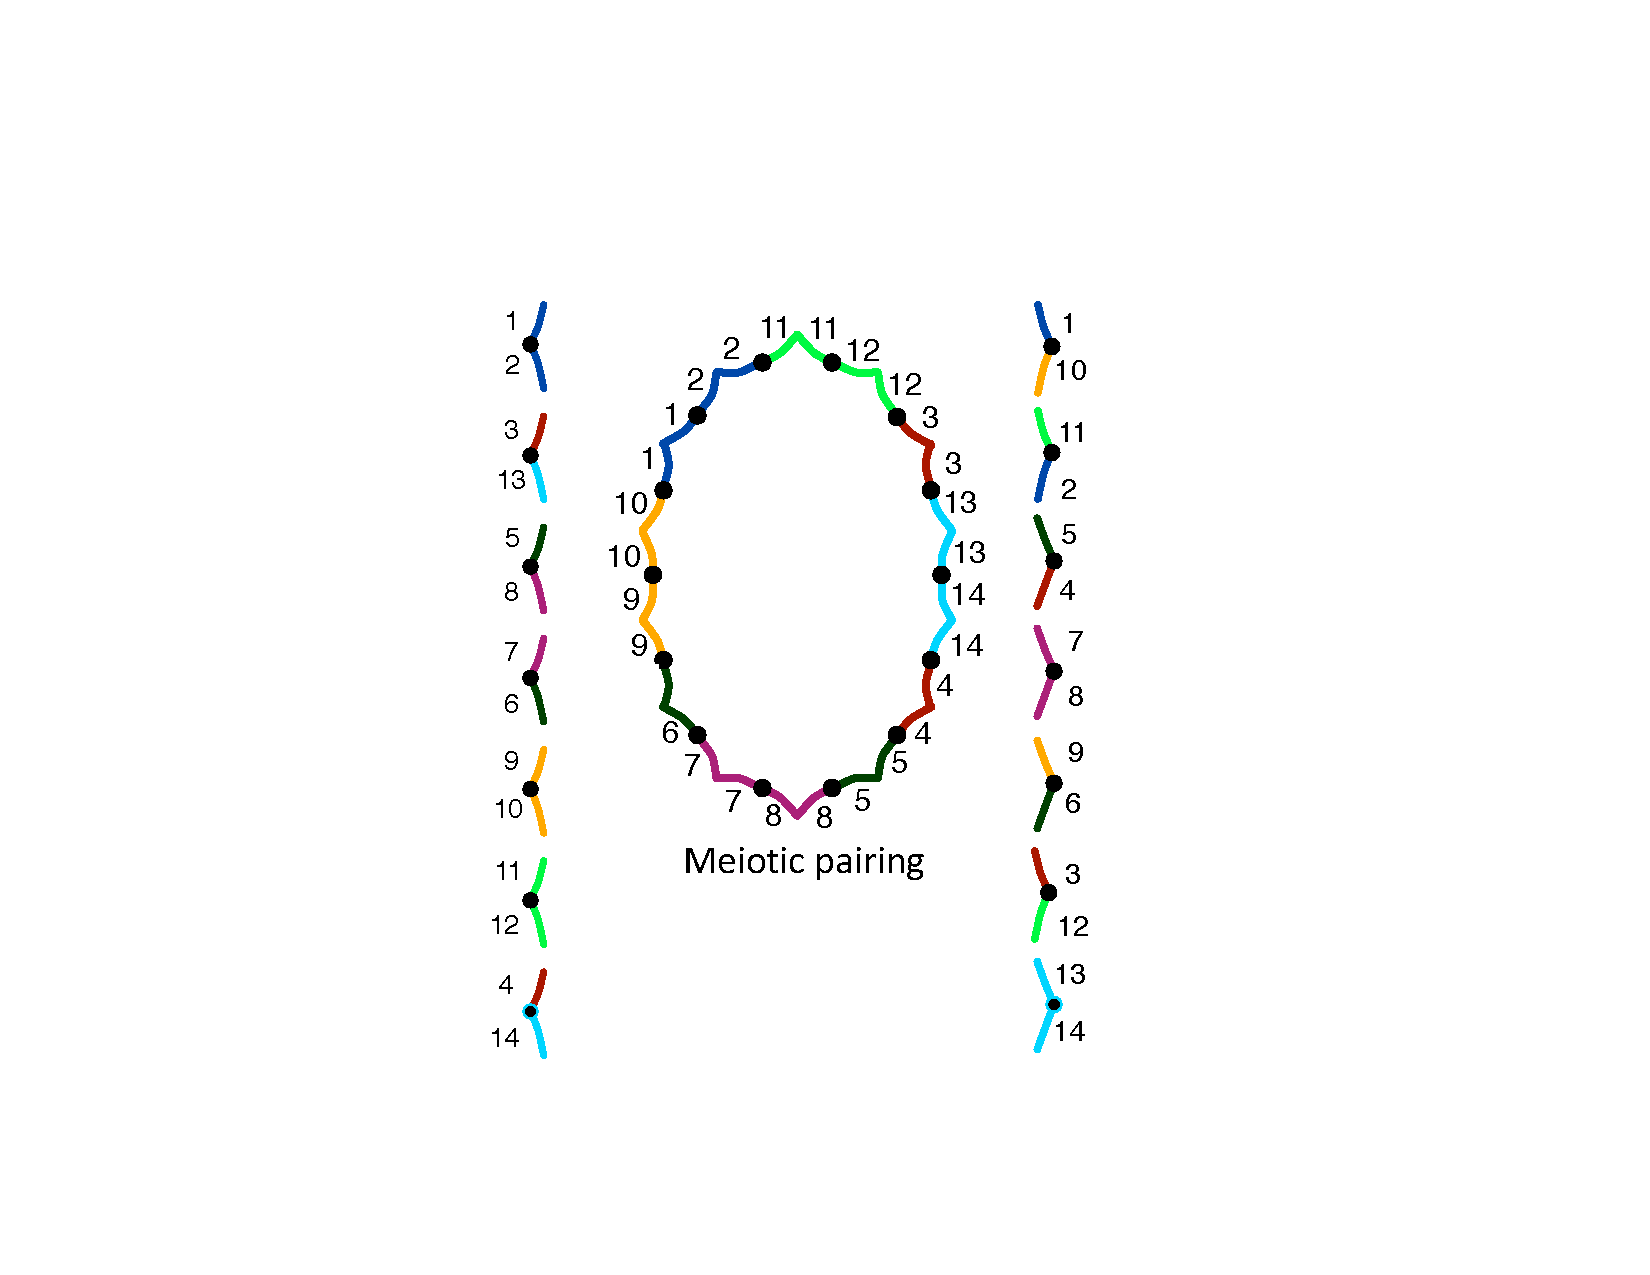
\includegraphics[width = \textwidth]{figures/Reciprocal_translocations_Hollister.pdf}
\end{center}
\caption{A schematic diagram of the karotype of an evening primrose. The two columns show a heterozygote individual's diploid chromosomal complement. Each chromosome is heterozygote for two different translocations. For example both the top-most chromosomes has one arm from chromosome 1, but the other arm is heterozygote for a large translocation from the ancestral chromsome 2 and 10. Due to these translocations the meiotic pairing form a complete ring of chromosomes, which prevent crossing over and independent segregation. Thanks to Jesse Hollister for this image. } \label{}  %é
\end{marginfigure}

In the Evening primrose genus ({\it Oenothera}), there are a number of young, independently-derived, asexual species. In each species this asexuality is due to a complicated series of reciprocal translocations which prevent recombination and segregation and ensure that every plant is permanently-heterozygote for these rearrangements due to lethality. This system is quite complicated, and super cool. We don't need to worry about the details but importantly each species is functionally asexual. \citet{hollister2014recurrent} sampled transcriptome data from across the Evening primrose clade, and took advantage of 7 independent, asexual-sexual sister pairs of species to examine the impact of the evolution of asexuality for molecular evolution.  
\begin{figure}
\begin{center}
  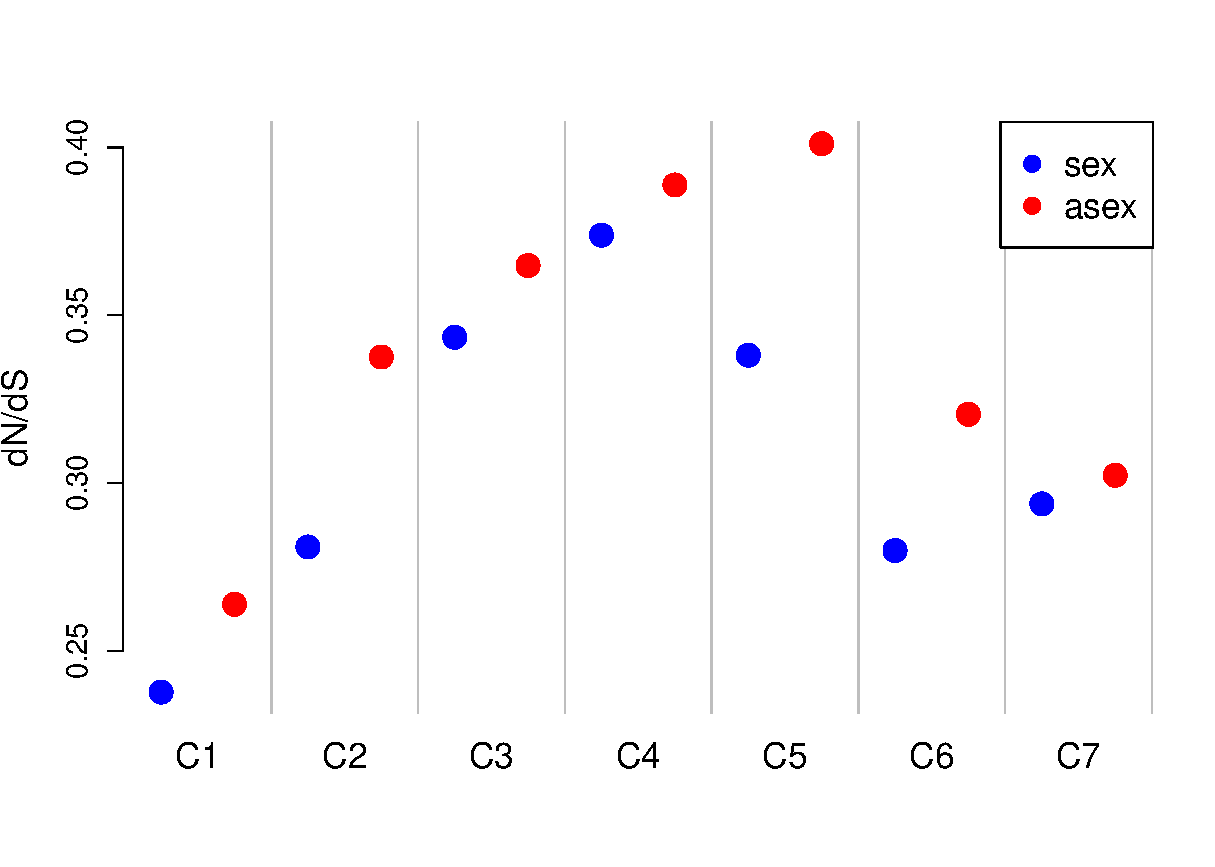
\includegraphics[width = 0.8 \textwidth]{Journal_figs/recom_selection/evening_primrose/evening_primrose_omega.pdf}
\end{center}
\caption[][4cm]{$\dNdS$ calculated on sexual (circles) and asexual (diamonds) lineages of each of seven sister pairs of species. Data from \citet{hollister2014recurrent}. \gitcode{https://github.com/cooplab/popgen-notes/blob/master/Journal_figs/recom_selection/evening_primrose/evening_primrose_omega.R}| } \label{fig:evening_primrose_omega}  %é
\end{figure}

The $\dNdS$ for the sexual and asexual species for each of the seven pairs (C1-C7) is shown in Figure \ref{fig:evening_primrose_omega}. In every pair $\dNdS$ is higher in the asexual species. The genomes of the asexual species are evolving in a less constrained fashion, likely due to weakly deleterious mutations accumulating due to hitchhiking with beneficial alleles and the slow crank of Muller's ratchet. 
\begin{marginfigure}[0cm]
\begin{center}
  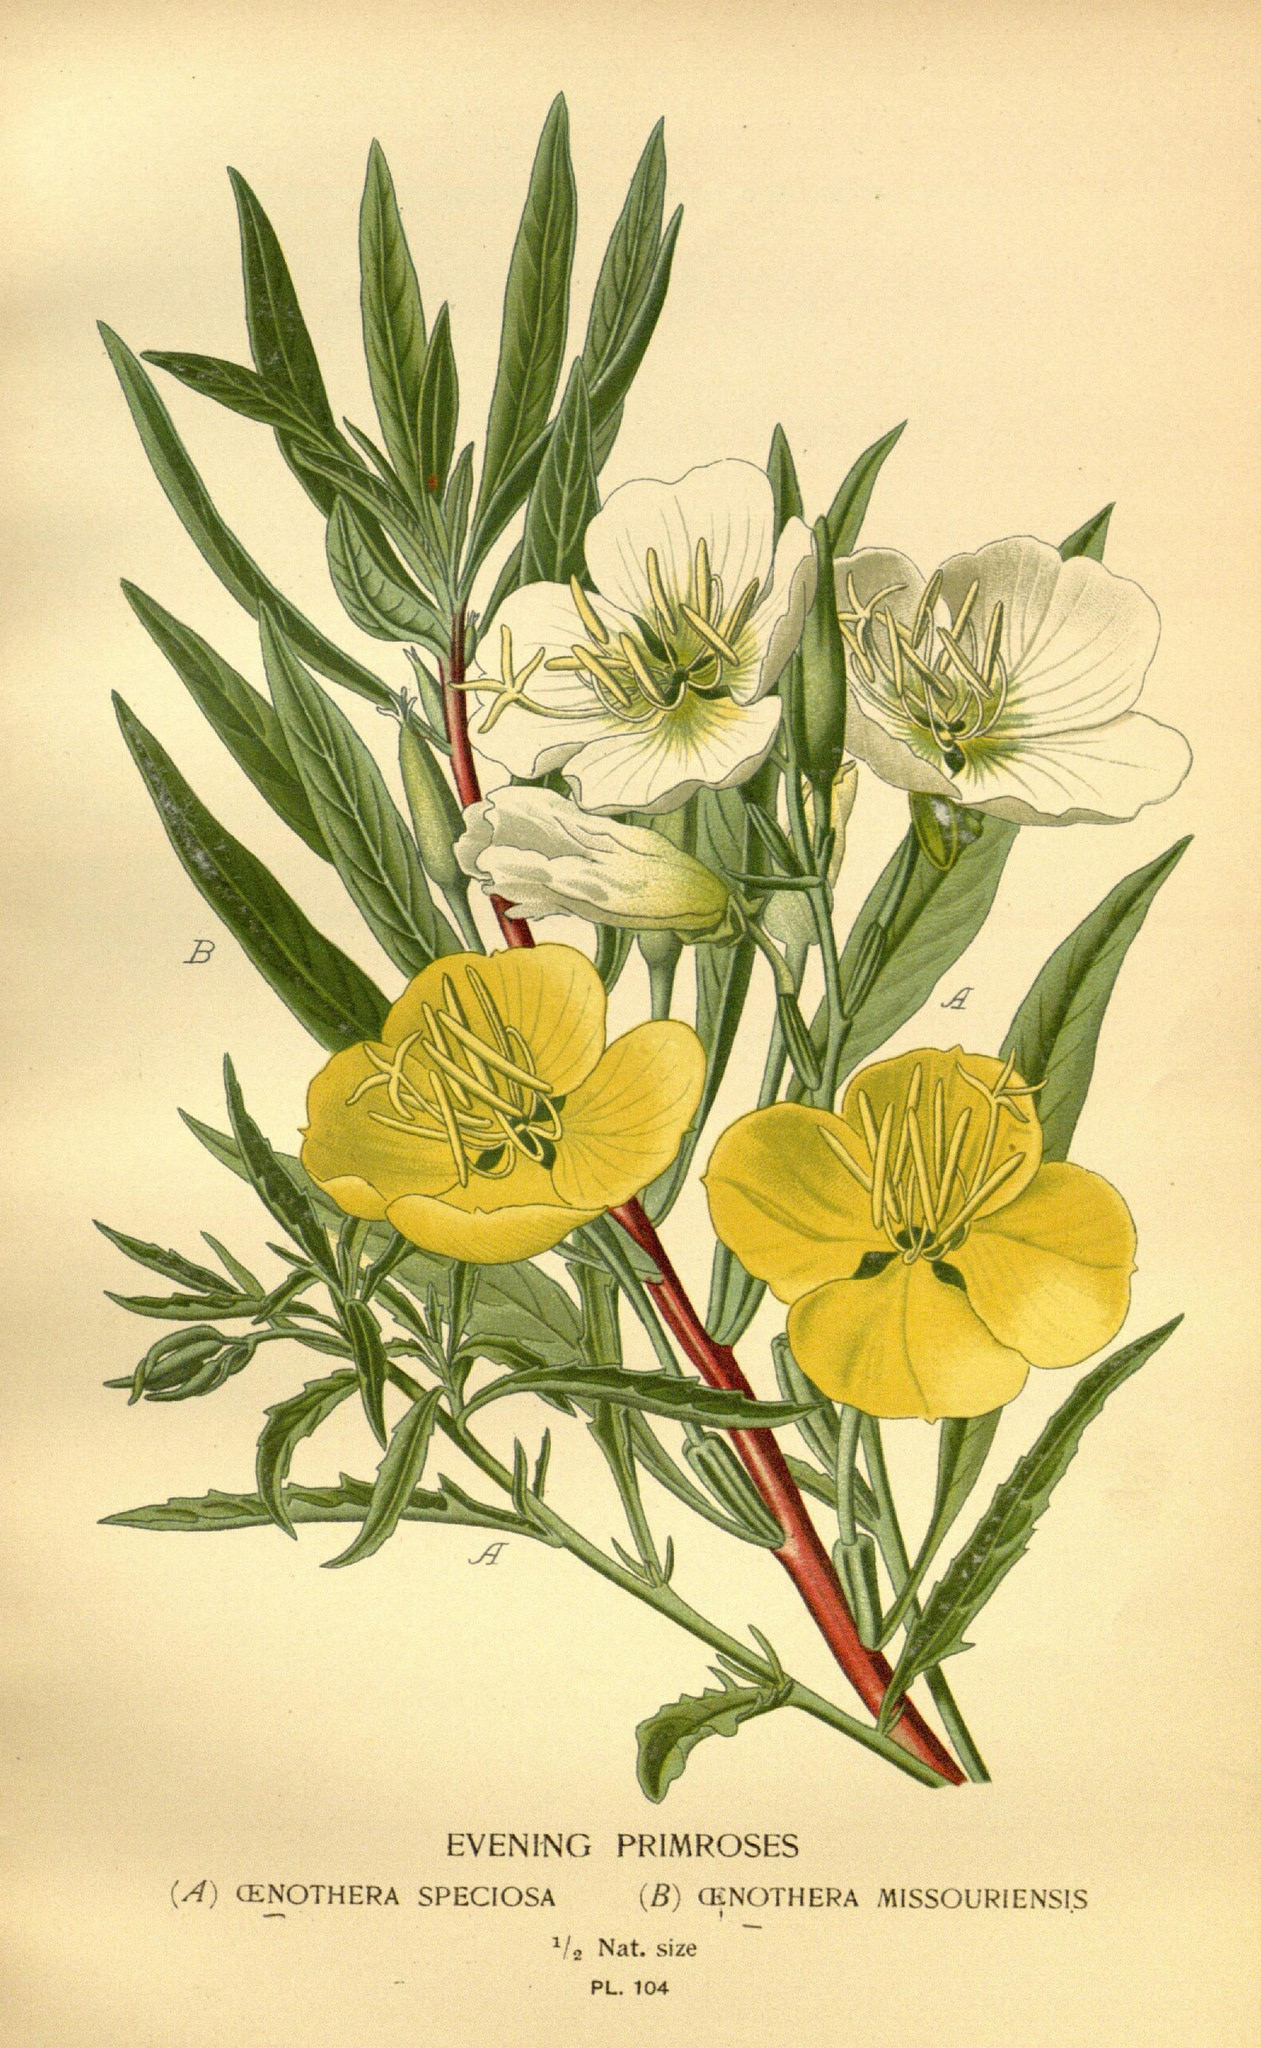
\includegraphics[width = \textwidth]{illustration_images/multiple_sel_loci/Evening_primrose/10575005313_f2c8839a80_k.jpg}
\end{center}
\caption{ Showy evening primrose ({\it Oenothera speciosa}), the sexual species in the clade C2 from Figure \ref{fig:evening_primrose_omega}. \BHLCC{Favourite flowers of garden and greenhouse (1896). Step, E. }{https://www.flickr.com/photos/61021753@N02/10575005313/}{Missouri Botanical Garden}{2.0} } \label{}  %é
\end{marginfigure}

\paragraph{The maintainance of combinations of alleles in the face of recombination.}


In some cases balancing selection may be attempting to maintain multiple combinations of alleles in the population that work well together. However, recombination may be constantly ripping those alleles away from each other making it difficult to maintain these alleles. This can select for the supression of recombination. Some of the most dramatic demonstrations of this tension involve the evolution of so-called super genes. We'll first consider the evolution of a mimicry supergene in {\it Heliconius numata} as an example of this.  

Some of the most spectacular examples of M{\"u}llerian mimicry in the world are found in {\it Heliconius} butterflies. These butterflies are unpalatable to predators, and different species mimic each other so benefiting from not being eaten by predators, which rapidly learn to avoid all these species). In many of these species multiple mimicry morphs are found as we move across geographic space. In  {\it Heliconius numata} a number of different morphs mimic morphs from a distantly related {\it Melinaea} species. 

\begin{figure} %[0cm]
\begin{center}
  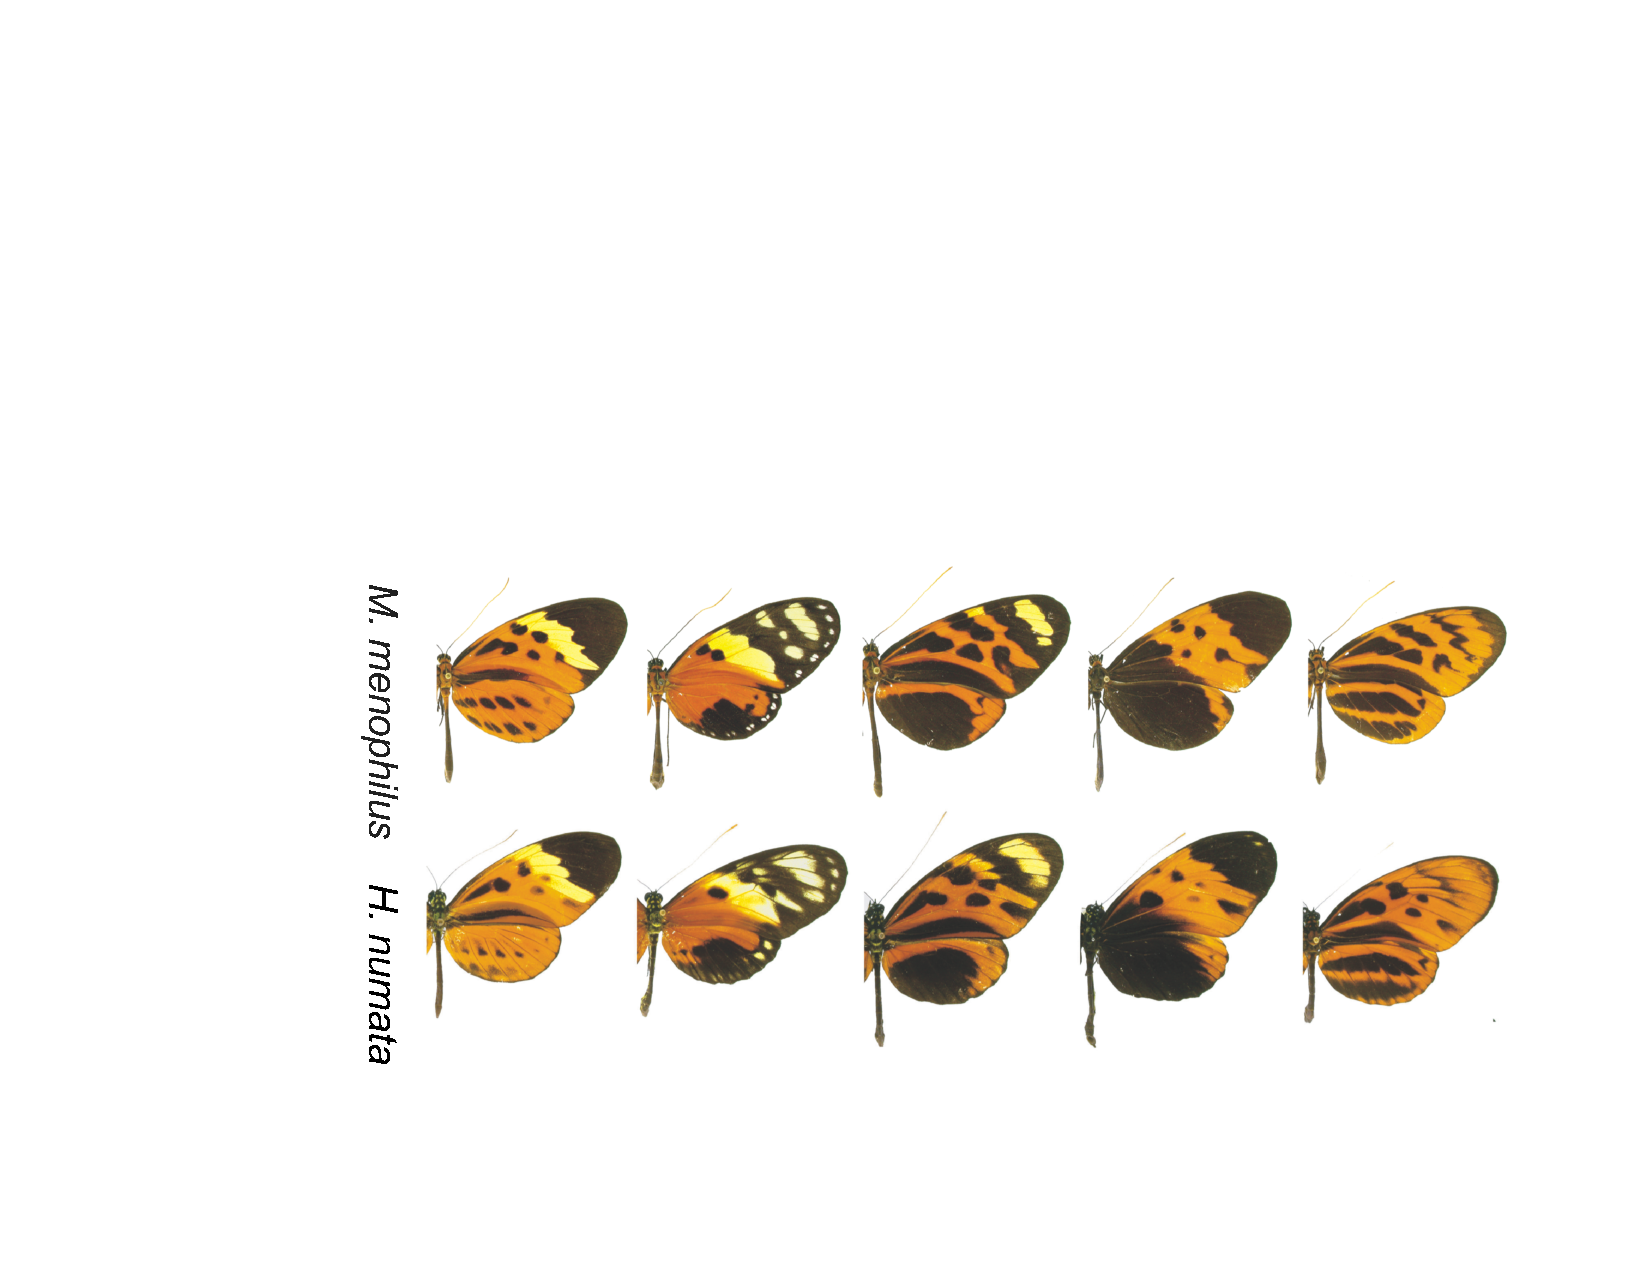
\includegraphics[width = \textwidth]{Journal_figs/recom_selection/H_numata/H_numata.pdf}
\end{center}
\caption{Five sympatric forms of {\it H. numata} from northern Peru, and their distantly related comimetic Melinaea species.  First row: {\it M. menophilus ssp. nov., M. ludovica ludovica, M. marsaeus rileyi, M. marsaeus mothone, and M. marsaeus phasiana}. Second row, {\it H. n. f. tarapotensis, H. n. f. silvana, H. n.f. aurora, H. n.f. bicoloratus, and H. n. f. arcuella}. Figure and caption from \citet{joron2006conserved} cropped, \PLOSccBY. } \label{}  %é
\end{figure}

To keep things relatively simple lets focus on two differences between  {\it silvana} and {\it  bicoloratus}, the yellow stripe on the top wing of {\it silvana} and the black bottom wing of  {\it  bicoloratus}. Lets imagine that these two differences are due to a simple two locus system. The first locus segregates for Y/y, where the Y allele encodes for a top-wing yellow band, and y encodes for the absence of the yellow band. The second locus segregates for B/b where B encodes for the bottom-wing being black, and b for the absence of black on the bottom wing. If Y is recessive and B is dominant, then the silvana phenotype corresponds to a YY bb genotype. Due to the dominance of the y and B alleles the bicoloratus phenotype can be achieved by various genotypes (Yy Bb, yy BB, Yy BB, yy Bb).  Both of these phenotypes offer an advantage as they mimic a {\it M. menophilus} model. But there are also genotypes that don't do as well; YY BB individuals have a yellow band and a black bottom and so don't do a great job mimicing anything and so will be eaten. Thinking about the  four possible haplotypes, y-B has high marginal fitness as due to its combo of dominant alleles it'll always produce a bicoloratus phenotype. Likewise the Y-b haplotype has high marginal fitness, as it does well in the homozygous state ({\it silvana} phenotype), and when it is paired with the y-B allele. However, the Y-B and y-b haplotypes fair less well as they carry two alleles that don't work well with each other and so are often individuals who suffer high rates of predation. 

\begin{figure} %[0cm]
\begin{center}
 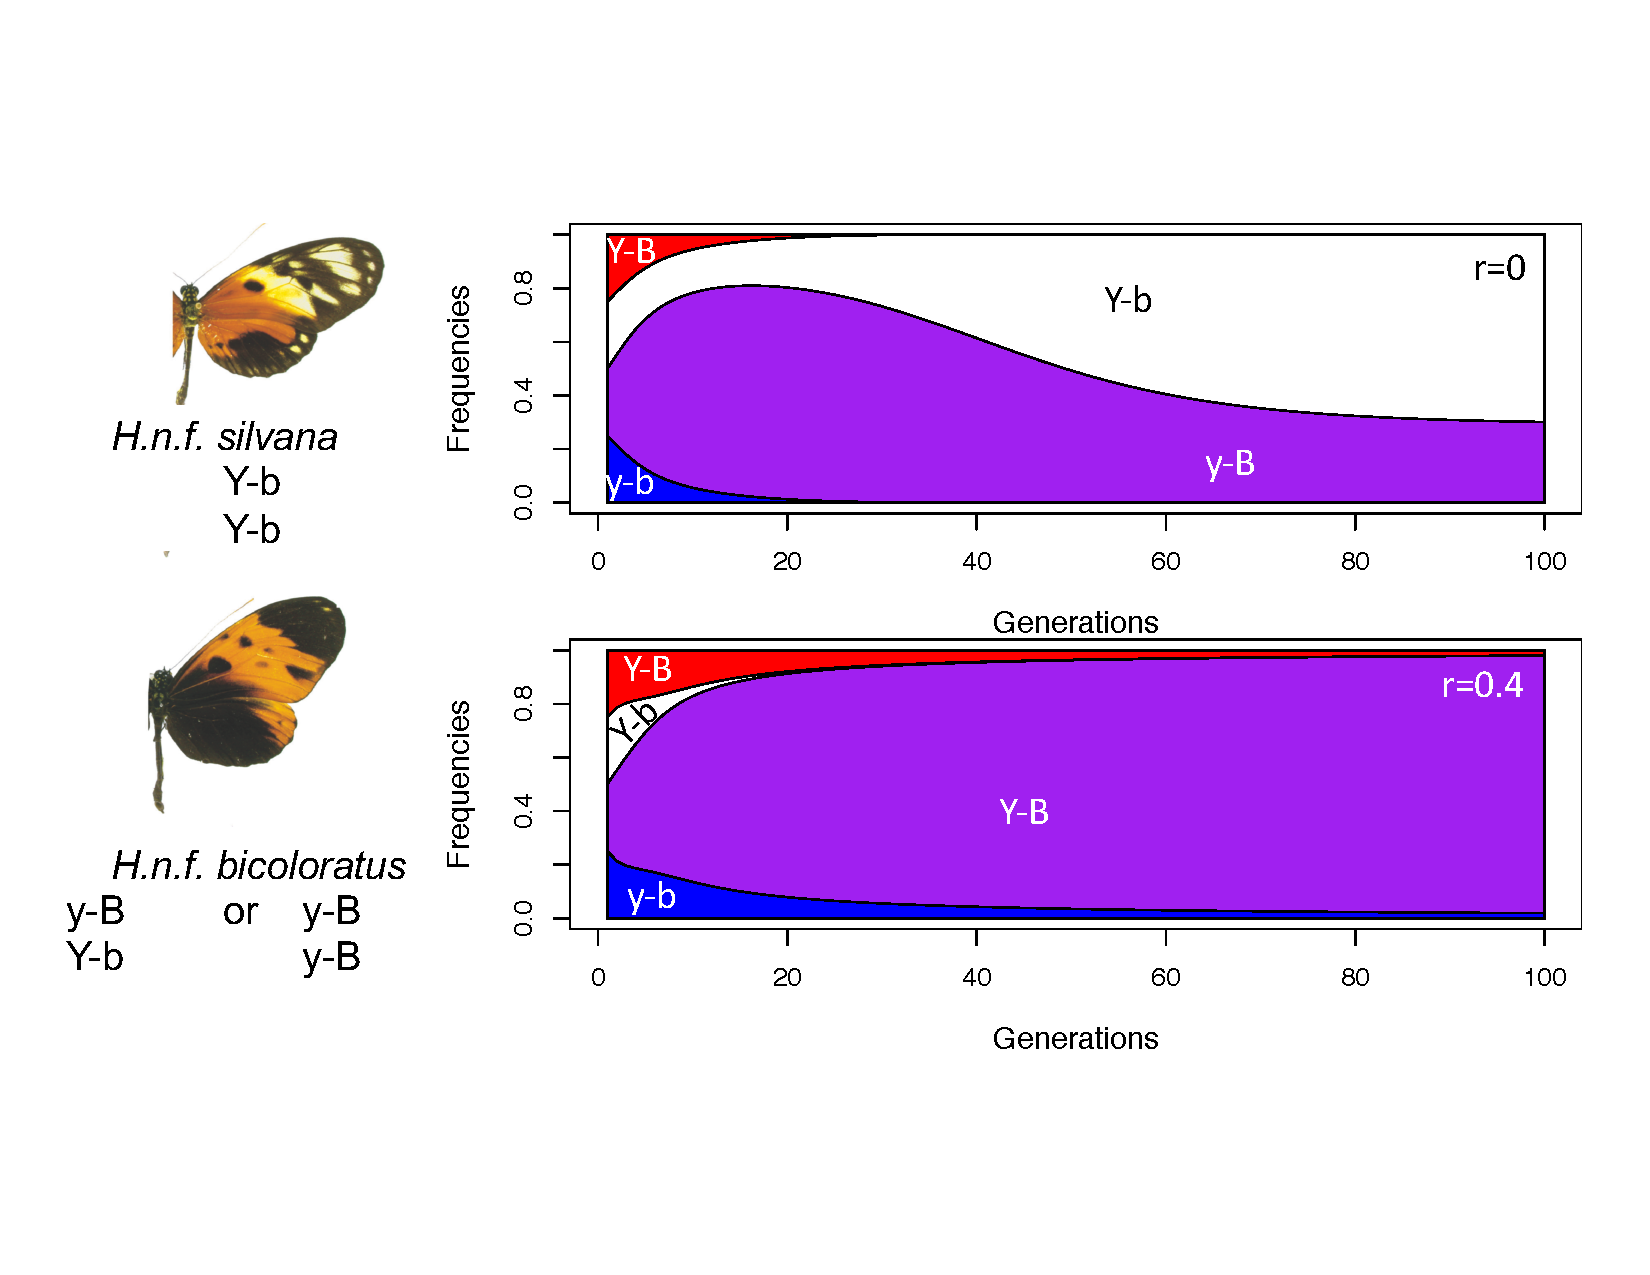
\includegraphics[width = \textwidth]{figures/selection_recom_interaction/H_numata_two_loc_freqs.pdf}
\end{center}
\caption{ } \label{fig:numata_two_loc_freqs}  %é
\end{figure}

If no recombination occurs between these loci ($r=0$, Figure \ref{fig:numata_two_loc_freqs}), then the Y-B and y-b are selected out of the population, and the y-B and and  Y-b can be stably maintained. However, when there's too much recombination between our loci (e.g. $r=0.4$, Figure \ref{fig:numata_two_loc_freqs}) the high-fitness haplotypes keep getting ripped apart by recombination and the Y-b is lost from the population as it's recessive advantage is lost as it's too often being broken up by recombination in heterozygotes.

\paragraph{Supergenes to the rescue!}

So our polymorphisms can only be maintained if they are tightly linked, i.eif these alleles arose at loci that are genetically close to each other. But how is it possible that these alleles arose close to each other? Well the trick is that they don't necessarily have to arise very close to each other. If such a system is polymorphic but being regularly broken up by recombination, a chromosomal inversion--the flipping around of a whole section of chromosome-- can arise and will supress recombination. Imagine that our two loci are far apart genetically, and a chromosomal inversion arises on the Y-b  background forming the b-Y haplotype. This inverted haplotype will not recombine with the y-B haplotype when it is present in a heterozygote, thus it is not broken down by recombination. This inverted haplotype, which enjoys the fitness benefits of the Y-b, can therefore replace the Y-b haplotype in the population. The two other low fitness haplotypes will disappear as they sre no longer being generated by recombination, leaving just the y-B and b-Y. \marginnote{\begin{quote}
``coadapted combinations of several or many genes locked in inverted sections of chromosomes and therefore inherited as single units.''
\citet{dobzhansky1970genetics} on supergenes. 
\end{quote} }
  The polymorphism system now behaves like alleles at a single locus, a super gene  (e.g. like $r=0$ in Figure \ref{fig:numata_two_loc_freqs}).

  Now the {\it H. numata} system is vastly more complicated than our toy two locus system, presumably involving many changes and refinements, but the same principle holds \citep{joron2011chromosomal}. The differences between the different {\it H. numata} mimmicy morphs is found on a single chromosome, and the inheritance behaves as if controlled by a single locus (albeit with many alleles).  The {\it H. n. f. silvana} individuals carry a recessive haplotype of alleles that which is known to be locked together by a $\sim 400$kb inversion, that is a different chromosomal orientation from the {\it bicoloratus} allele (haplotype) which acts as a dominant allele. Other alleles at this same chromosomal region provide the genetic basis of the other morphs, and sometimes correspond to further inversions with a range of dominance relationships. 


\begin{figure} %[0cm]
\begin{center}
\includegraphics[width = \textwidth]{Journal_figs/recom_selection/Mimulus_inversion/annual_perennial_fitness.pdf}
\end{center}
\caption{{\bf Left)} A coastal perennial and an Inland annuals {\it Mimulus gutatus} \citet{lowry2010widespread}, image from \citet{lowry2010widespread} \PLOSccBY. {\bf Right)} A reciprocal transplant experiment showing that coastal perennial and an Inland annuals are locally adapted to their respective habitats. Data from  \citet{lowry2010widespread}, \gitcode{https://github.com/cooplab/popgen-notes/blob/master/Journal_figs/recom_selection/Mimulus_inversion/annual_perennial_fitness.R}. 
}\label{fig:annual_perennial_fitness}
\end{figure}


\paragraph{Local Adaptation, Speciation, and Inversions.}
Inversions have long been thought to play an important role in local adaptation and speciation.
One example of an inversion underlying local adaptation occurs in {\it Mimulus gutatus},  in Western North America, where there are annual and perennial ecomorphs. 
The perennial form grows in many places along the Pacific coast, and in other places with year around moisture; it invests a lot of resources in
achieving large size and laying down resources for the next year, and as a result flowers late. The annual form grows inland, e.g. the California central valley,
where it has to invest all its effort in flowering rapidly before the long, hot, dry summer. Neither ecomorph does well in the other's environment. The perennials get crisped
before they have a chance to flower, while the annuals suffer from high rates of herbivory and cannot tolerate the salt spray.
\citet{lowry2010widespread} found that large inversion controled a lot of of the phenotypic variation in
flowering time and a range of other morphological differences between these two morphs. They also showed that the inversion controled a reasonable proportion of the
differences in fitness in the field, consistent with it underlying the fitness tradeoffs involved in local adaptation.
\begin{marginfigure} %[0cm]
\begin{center}
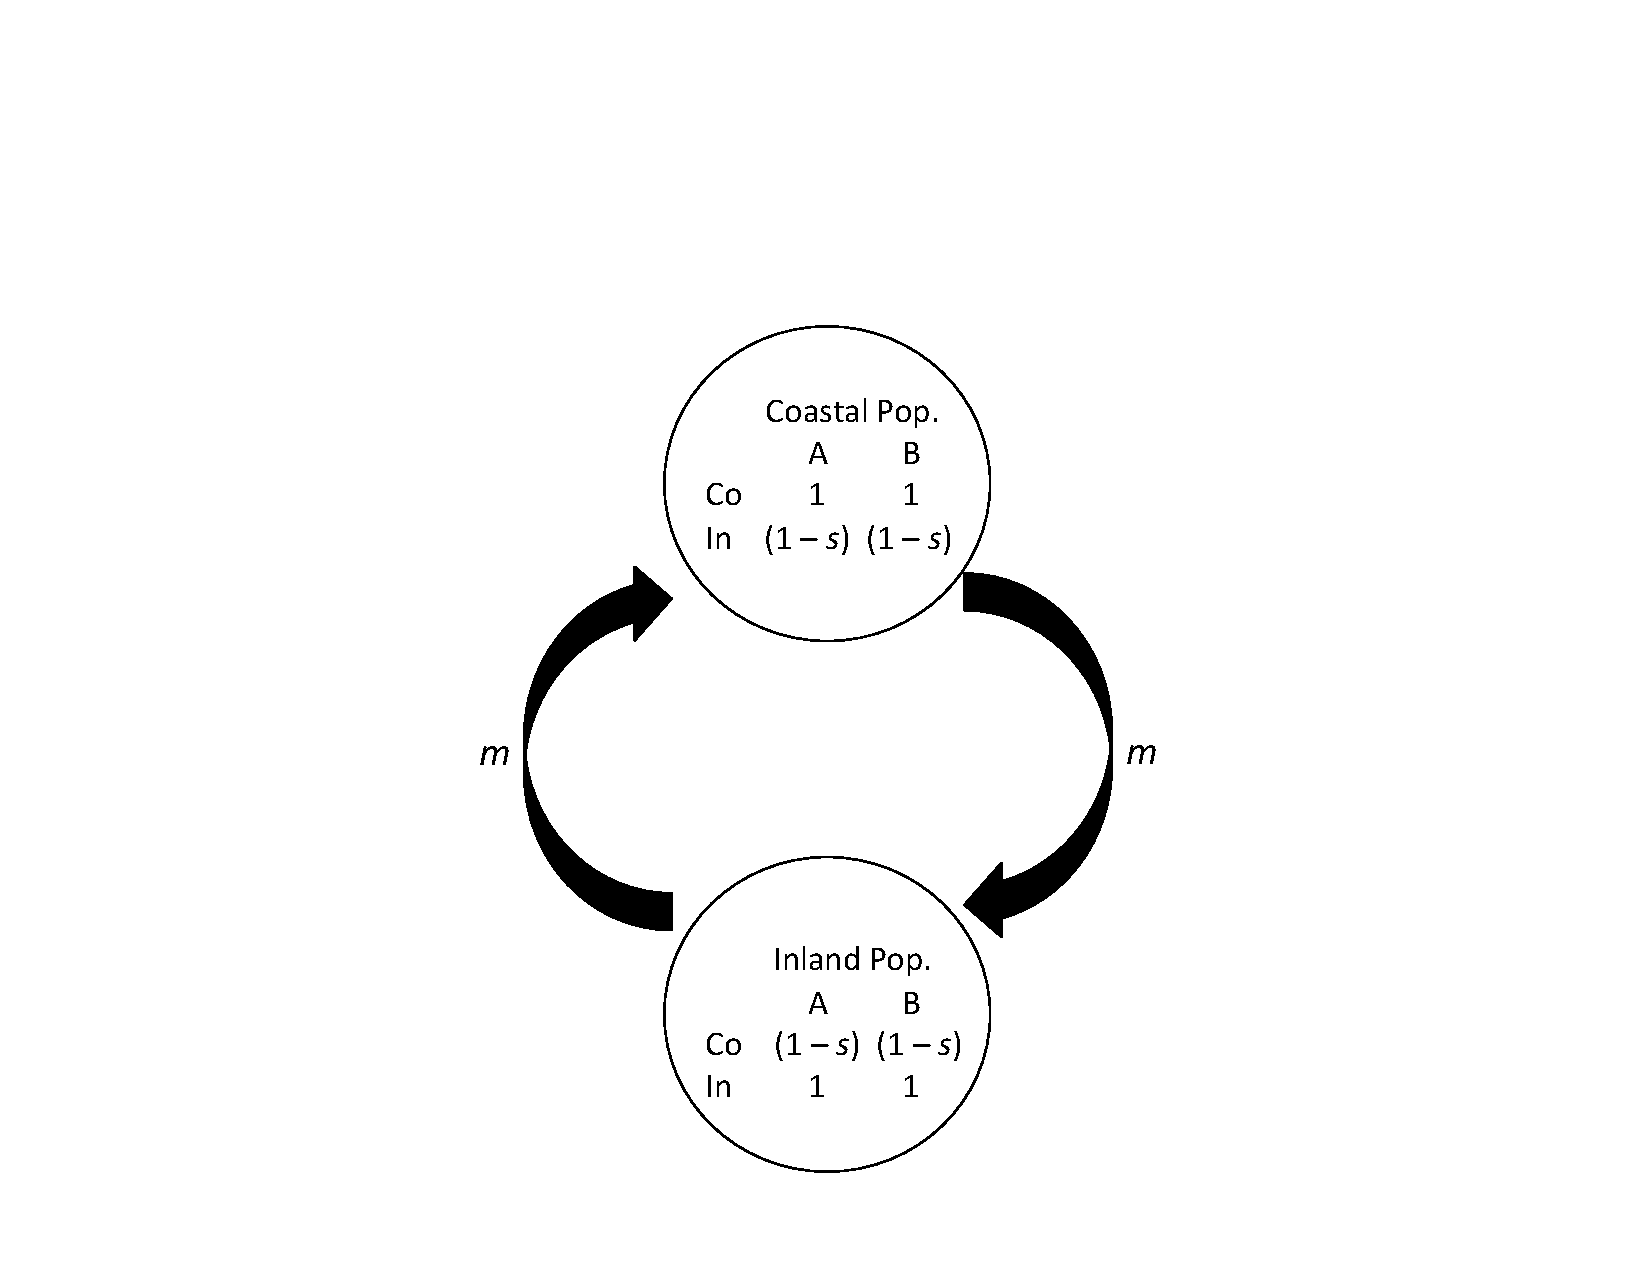
\includegraphics[width = \textwidth]{figures/inversion_mig_sel_balance.pdf}
\end{center}
\caption{A two locus, two population migration-selection balance system. Two loci A and B segregate for an Inland and Coastal adapted alleles.}
\end{marginfigure}
Why would an inversion be involved in locking together local adapted alleles? The basic idea, like above, is an inversion can be selected for we have two (or more) loci segregating for locally adapted alleles. Locally advantagous haplotypes are in danger of being broken up by recombination with maladapted haplotypes, which are constantly being
introduced into each population by migration from the other. If an inversion arises that locks these alleles together in one population, it can be selected for as does not suffer the ill effects from recombination with migrating maladaptive haplotype. 
 
  % In this simple model of viability selection

\subsection{Sex Chromosomes and the dynamics of selection and recombination.}
  \begin{marginfigure} %[0cm]
\begin{center}
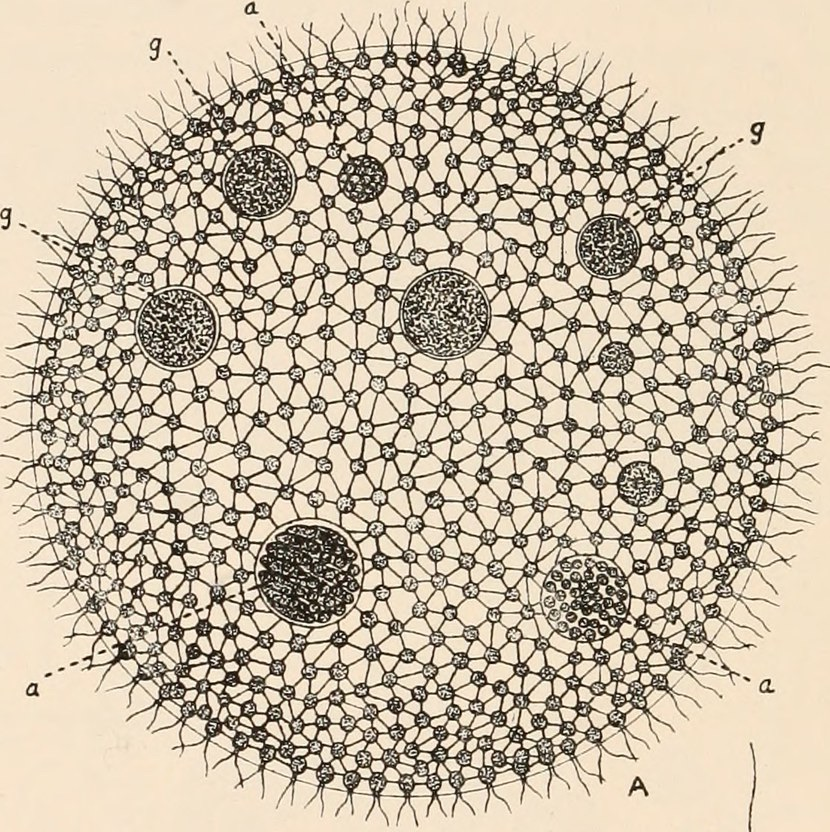
\includegraphics[width = \textwidth]{illustration_images/multiple_sel_loci/volvox/volvox.jpg}
\end{center}
\caption{ {\it Volvox aureus}, Volvox are spherical, multicellular green algae. The surface is made up of a single layer of somatic cells (up to 50k cells) beating their flagella. Some species of Volvox have male and female gametes, being made in the germ cells (a and g respectively) in the middle of the sphere. Some Volvox have separate sexes, where different individuals produce male and female gametes.}
\end{marginfigure}
The production of different sized gametes (anisogamy) has arisen a number of times in multi-cellular life, with male and female gametes are defined by their relative sizes. The smaller, and often more mobile, gametes are defined male gametes  (e.g. sperm), while the larger, well provisioned, and often less mobile are defined as female gametes (e.g. egg cell). The evolution of anisogamy is thought to be due to disruptive selection due to a tradeoff pulling in opposite directions towards mobile gametes able to move further and in the opposite direction towards better provised gametes better able to build larger zygotes. In many organisms individuals can produce both male and female gametes, while some species have evolved separate sexes, likely in part as an inbreeding avoidance mechanism. There is huge diversity in sex determination mechanisms across the eukaryotic tree (Figure \ref{fig:Tree_of_sex}. This is all to say, that biology is wonderfully complicated. 
\begin{figure*} %[0cm]
\begin{center}
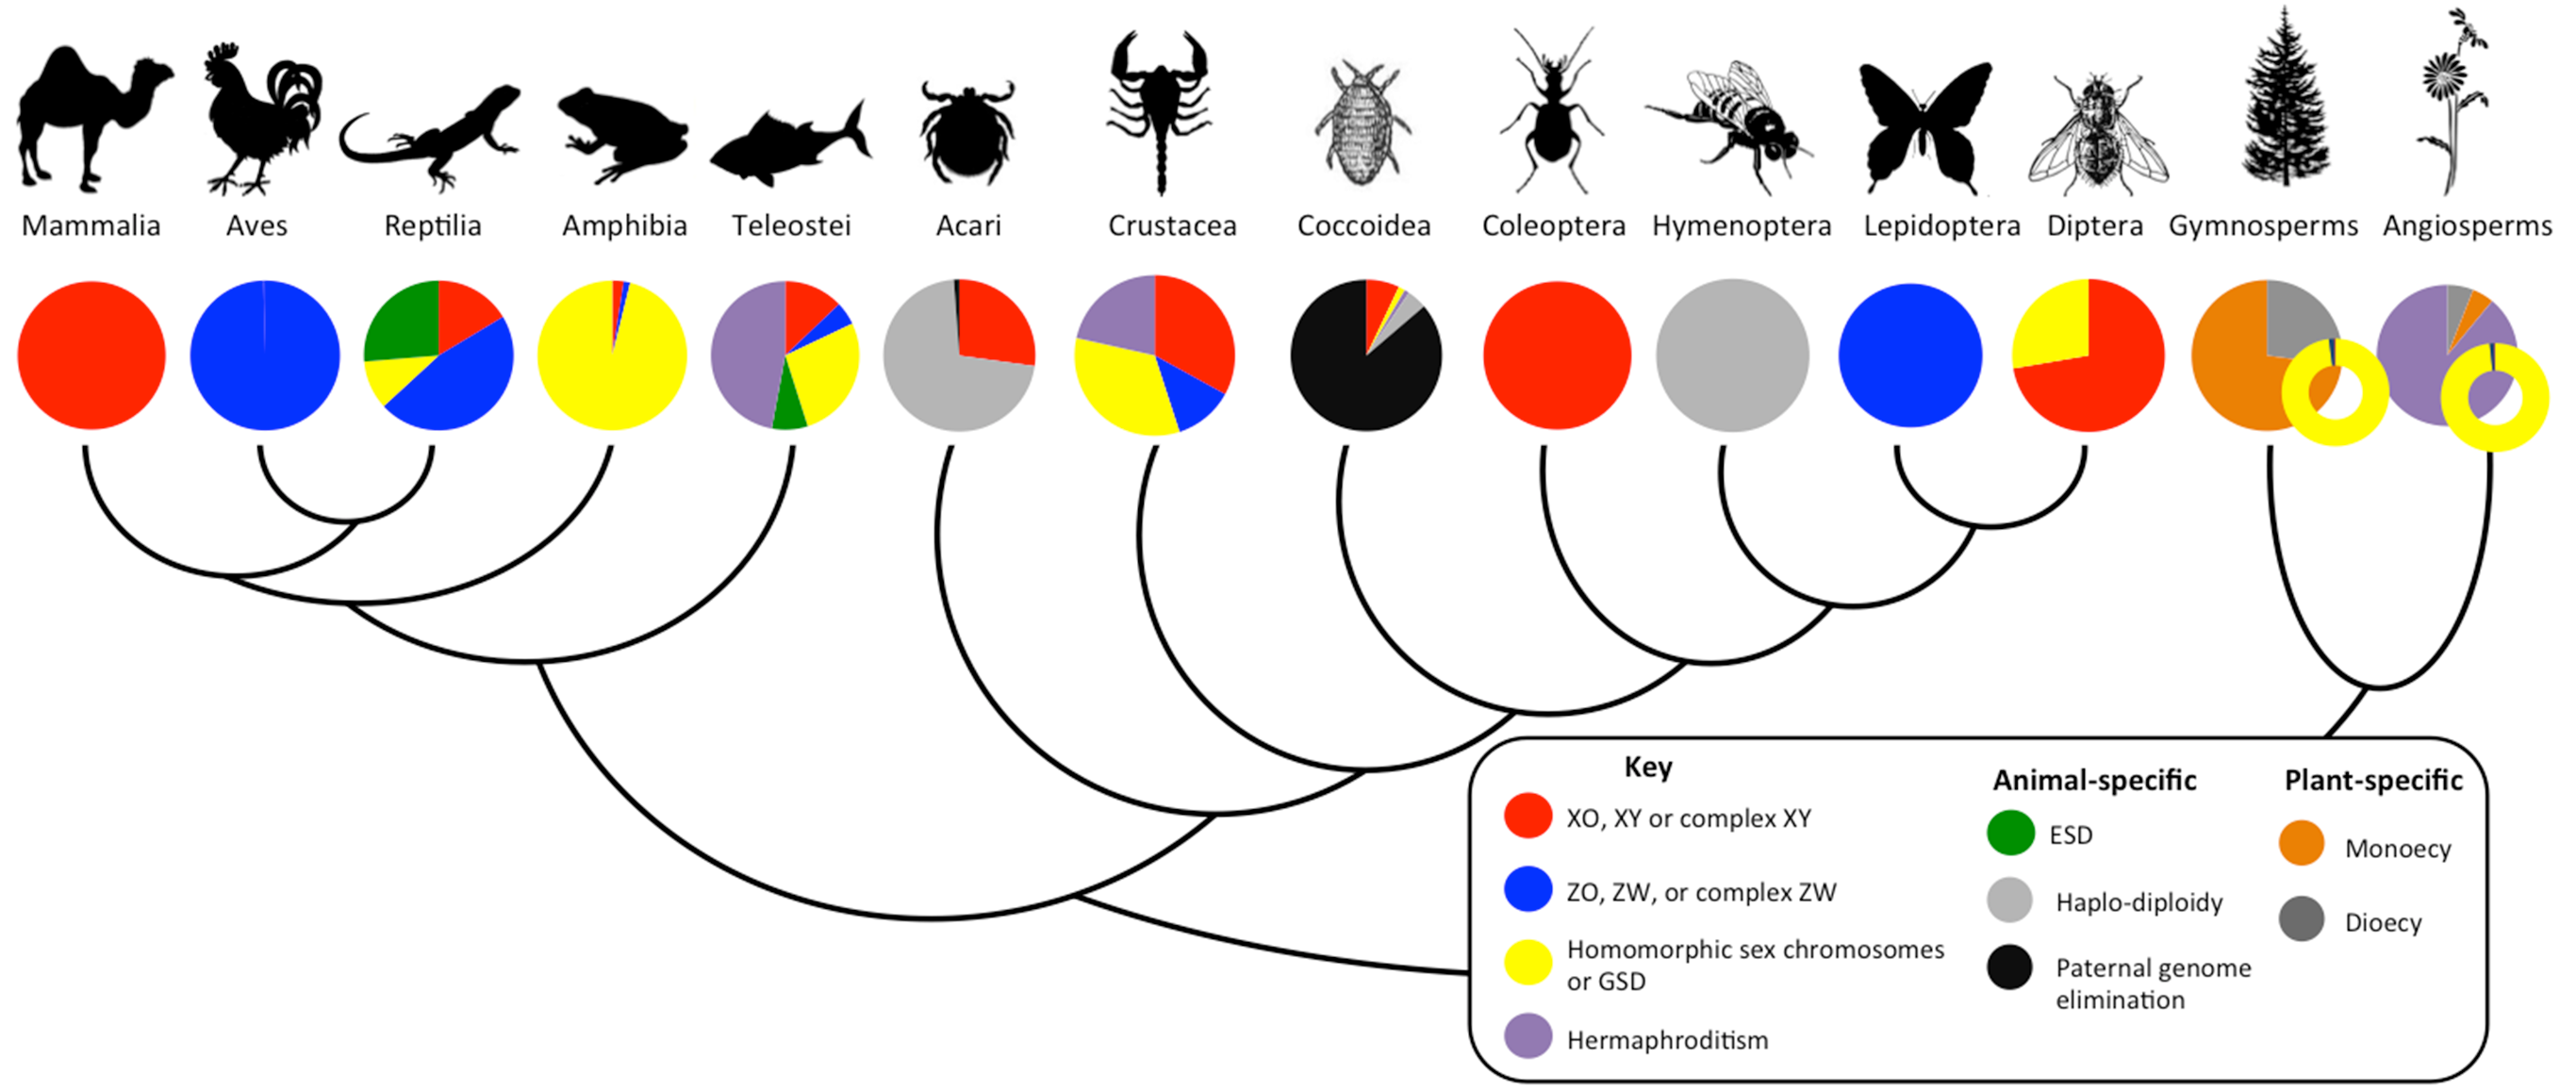
\includegraphics[width = \textwidth]{Journal_figs/recom_selection/Sex_determ_why_so_many_ways/Tree_of_sex.png}
\end{center}
\caption{Diversity of sex determination systems for representative plant and animal clades. Figure and caption from \citet{bachtrog2014sex}, \PLOSccBY. }  \label{fig:Tree_of_sex}
\end{figure*}


In mammals, and many over systems with genetic sex determination, the genes responsible for sex determination lie on a pair of heteromorphic sex chromosomes, i.e. pair of chromosomes that are quite different in size. In mammals it is the male determining Y chromosome that has a very small gene content compared to the X chromosome (Figure \ref{fig:XY_ZW}). But in other groups such as birds, and some snakes, females carry a gene poor W with males being the homogametic sex, carrying two Zs.  If you are still reading send Graham a picture of Nettie Stevens, she discovered sex chromosomes in 1905 \citep{stevens1905studies}. These examples of heteromorphic sex chromosomes, and many others like them, are thought to have arisen from an ancestral pair of autosomes? What then explains their evolution?
 \begin{marginfigure} %[0cm]
\begin{center}
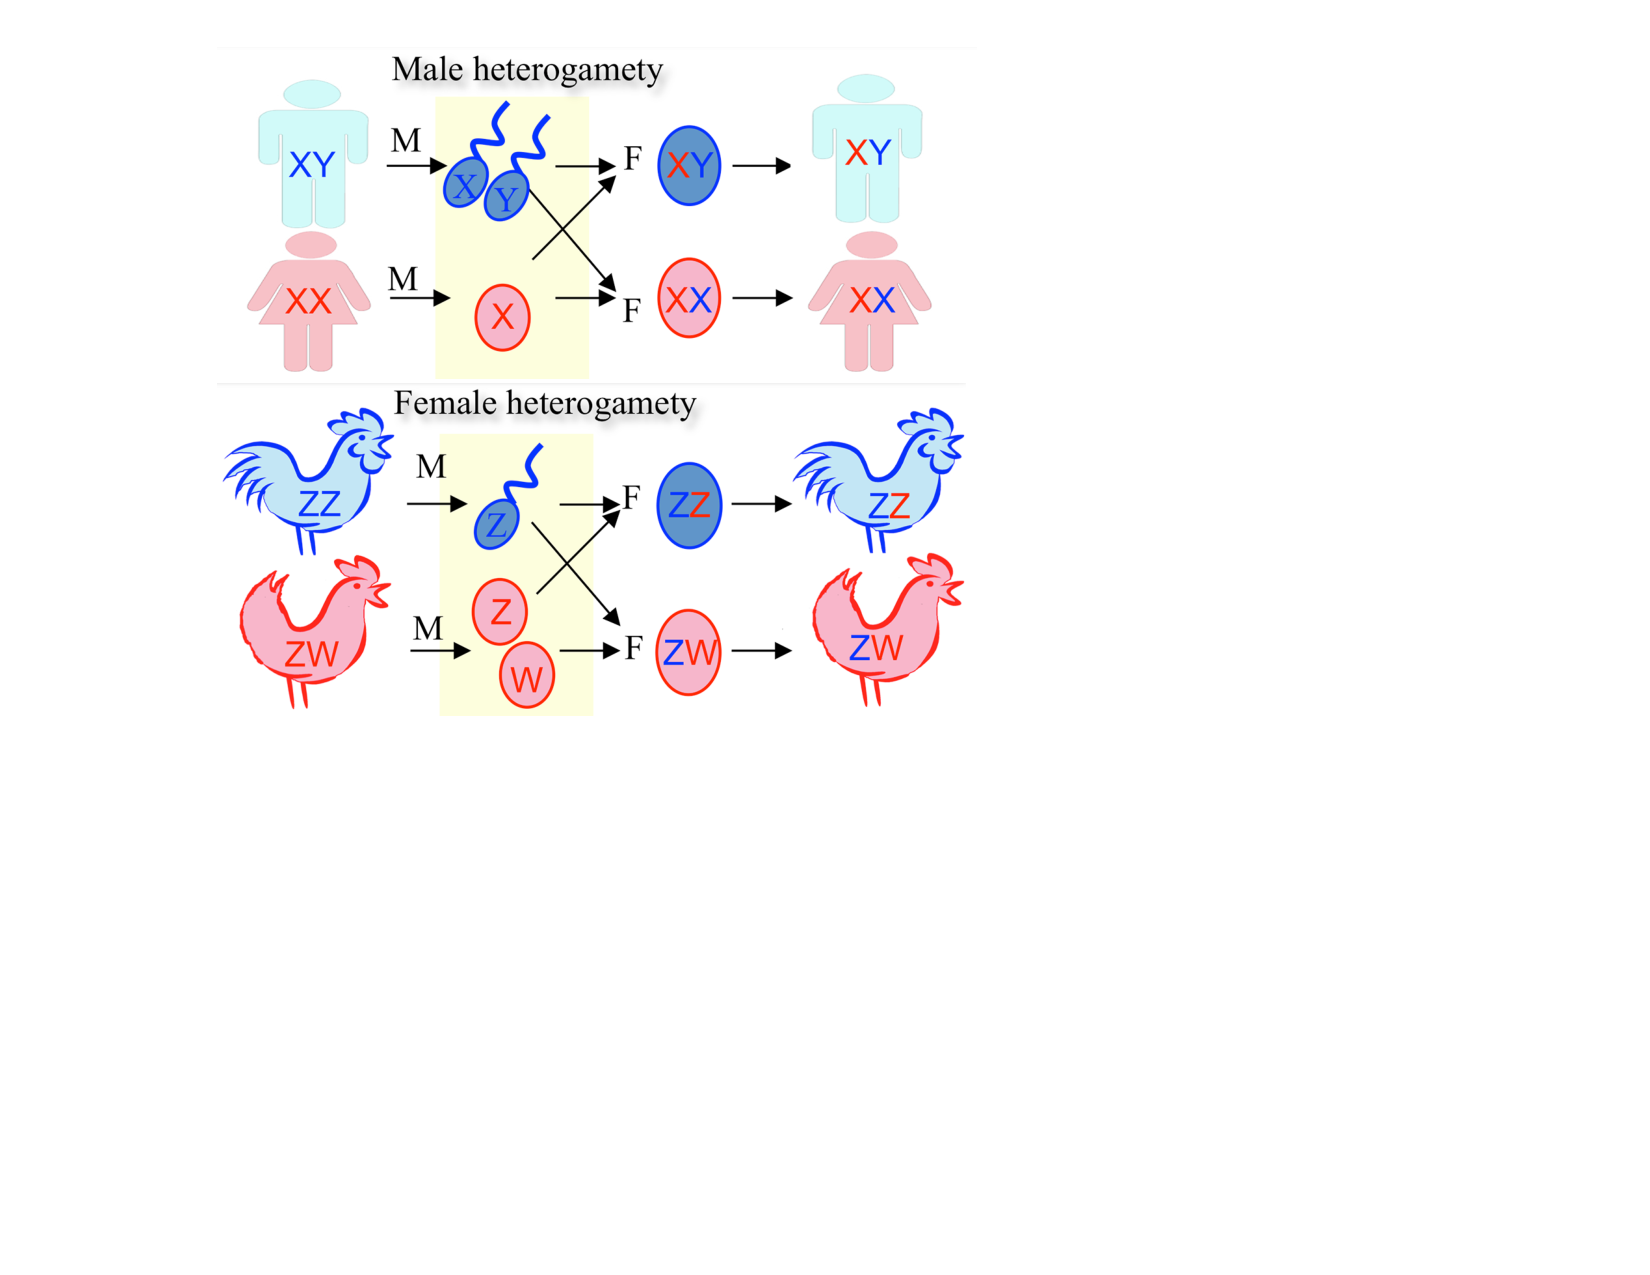
\includegraphics[width = \textwidth]{Journal_figs/recom_selection/Sex_determ_why_so_many_ways/XY_ZW_cartoon.pdf}
\end{center}
\caption{Figure from \citet{bachtrog2014sex}, \PLOSccBY cropped from original. }  \label{fig:XY_ZW}
\end{marginfigure}

A broad explanation for the evolution of sex chromosome goes as follows:\\


% https://journals.plos.org/plosbiology/article?id=10.1371/journal.pbio.1001643

In lake Malawi there are many very closely related cichlids species. In many of these species the males are brightly coloured to attracted females, while the females are often brown to help them avoid predators. In some of these species there is an alternative orange morph, called the marmalade cat morph, which are cryptic against the rocky bottom of the lake. This morph is due to a dominant \gc{(?)} mutation called OB at the pax7 \gc{(?)}, and the allele appears to shared across many of these species. This OB allele works well in females, however, in the males the OB allele disrupts their bright colouration. Thus the OB polymorphism is sexually antagonistic, i.e. it works well in females and poorly in males.

Males carrying the male-deleterious OB allele are rarely found, despite the allele being common in females. Why is that? Well because the OB allele is tightly linked to a newly emerged female-determining allele (W), with males carrying two copies of the Z allele. Males usually are homozygous for the ob-Z haplotype, while females can being either orange (OB-W/ob-Z) or brown (ob-W/ob-Z). Recombination between these two loci seems to be very rare, and so the sexually antagnostic allele OB appears to be mainly female specific. An inversion on the Z background would lock together the 

\begin{figure} %[0cm]
\begin{center}
\includegraphics[width = \textwidth]{figures/selection_recom_interaction/Cichlid_OB_sex_linkage.pdf}
\end{center}
\caption{ \newline \noindent \tiny{Image credits: Blue mbuna Male  {\it L. fuelleborni} by \href{https://commons.wikimedia.org/wiki/File:Labeotropheus_fuelleborni_in_Botanic_garden_in_Teplice_(2).JPG}{Chmee2}; % ( {\it Labeotropheus fuelleborni}).
  OB  Male {\it L. fuelleborni} by \href{https://de.wikipedia.org/wiki/Schabemund-Buntbarsch\#/media/File:Labeotropheus_fuelleborni_01.jpg}{Doronenko};
  Brown ob  {\it Tropheops} female by \href{https://www.flickr.com/photos/52993488@N03/4890217915}{Alexandra Tyers};
  Female  {\it L. fuelleborni} orange morph,  by \href{https://commons.wikimedia.org/wiki/File:Labeotropheus_fuelleborni1.jpg}{Mikko Stenberg} 
}}
\end{figure}
